% CVPR 2022 Paper Template
% based on the CVPR template provided by Ming-Ming Cheng (https://github.com/MCG-NKU/CVPR_Template)
% modified and extended by Stefan Roth (stefan.roth@NOSPAMtu-darmstadt.de)

\documentclass[10pt,twocolumn,letterpaper]{article}

%%%%%%%%% PAPER TYPE  - PLEASE UPDATE FOR FINAL VERSION
%\usepackage[review]{cvpr}      % To produce the REVIEW version
\usepackage{cvpr}              % To produce the CAMERA-READY version
%\usepackage[pagenumbers]{cvpr} % To force page numbers, e.g. for an arXiv version

% Include other packages here, before hyperref.
\usepackage{graphicx}
\usepackage{amsmath}
\usepackage{amssymb}
\usepackage{booktabs}


% It is strongly recommended to use hyperref, especially for the review version.
% hyperref with option pagebackref eases the reviewers' job.
% Please disable hyperref *only* if you encounter grave issues, e.g. with the
% file validation for the camera-ready version.
%
% If you comment hyperref and then uncomment it, you should delete
% ReviewTempalte.aux before re-running LaTeX.
% (Or just hit 'q' on the first LaTeX run, let it finish, and you
%  should be clear).
\usepackage[pagebackref,breaklinks,colorlinks]{hyperref}


% Support for easy cross-referencing
\usepackage[capitalize]{cleveref}
\crefname{section}{Sec.}{Secs.}
\Crefname{section}{Section}{Sections}
\Crefname{table}{Table}{Tables}
\crefname{table}{Tab.}{Tabs.}


%%%%%%%%% PAPER ID  - PLEASE UPDATE
\def\cvprPaperID{*****} % *** Enter the CVPR Paper ID here
\def\confName{CVPR}
\def\confYear{2022}


\begin{document}

%%%%%%%%% TITLE - PLEASE UPDATE
\title{Final Report on Flower Classification}

\author{Lujie Ma\\
University of Adelaide\\
School of Computer Science\\
{\tt\small a1810558@adelaide.edu.au}
% For a paper whose authors are all at the same institution,
% omit the following lines up until the closing ``}''.
% Additional authors and addresses can be added with ``\and'',
% just like the second author.
% To save space, use either the email address or home page, not both
\and
Wenlong Dai\\
University of Adelaide\\
School of Computer Science\\
{\tt\small a1777081@adelaide.edu.au}
}
\maketitle

%%%%%%%%% ABSTRACT
\begin{abstract}
   Classification is become more and more popular in our daily life, and gradually become more useful.
   Image classifier can do lots things for us, e.g. determining people's gender, identifying colors for special populations.
   To achieve this, we can use deep learning model trained on the specific data set.
   
\end{abstract}

%%%%%%%%% BODY TEXT

%------------------------------------------------------------------------
\section{Introduction}
In this project, we implemented the recognition of five types of flowers which are daisy, dandelion, rose, sunflower and tulip.
By using the base line model, the test accuracy is close to 71.3\% and getting overfitting.
Through our effort, the final accuracy can reach 92.6\% by adopting the deeper network resnet18.

%------------------------------------------------------------------------
\section{Before the start}

Here shows some works before starting the project.

%------------------------------------------------------------------------
\subsection{Review the dataset}

By checking the dataset, we notice that the number of pictures under each category is close to 400.
As shown in the Figure 1, we can see that although in the same category, there also has the huge difference which will influence the accuracy.
Such as the second picture of sunflower, the woman actually occupy most of the entire picture.

%---- figure part -------
\begin{figure}[htp]
  \centering
  %\fbox{\rule{0pt}{2in} \rule{0.9\linewidth}{0pt}}
   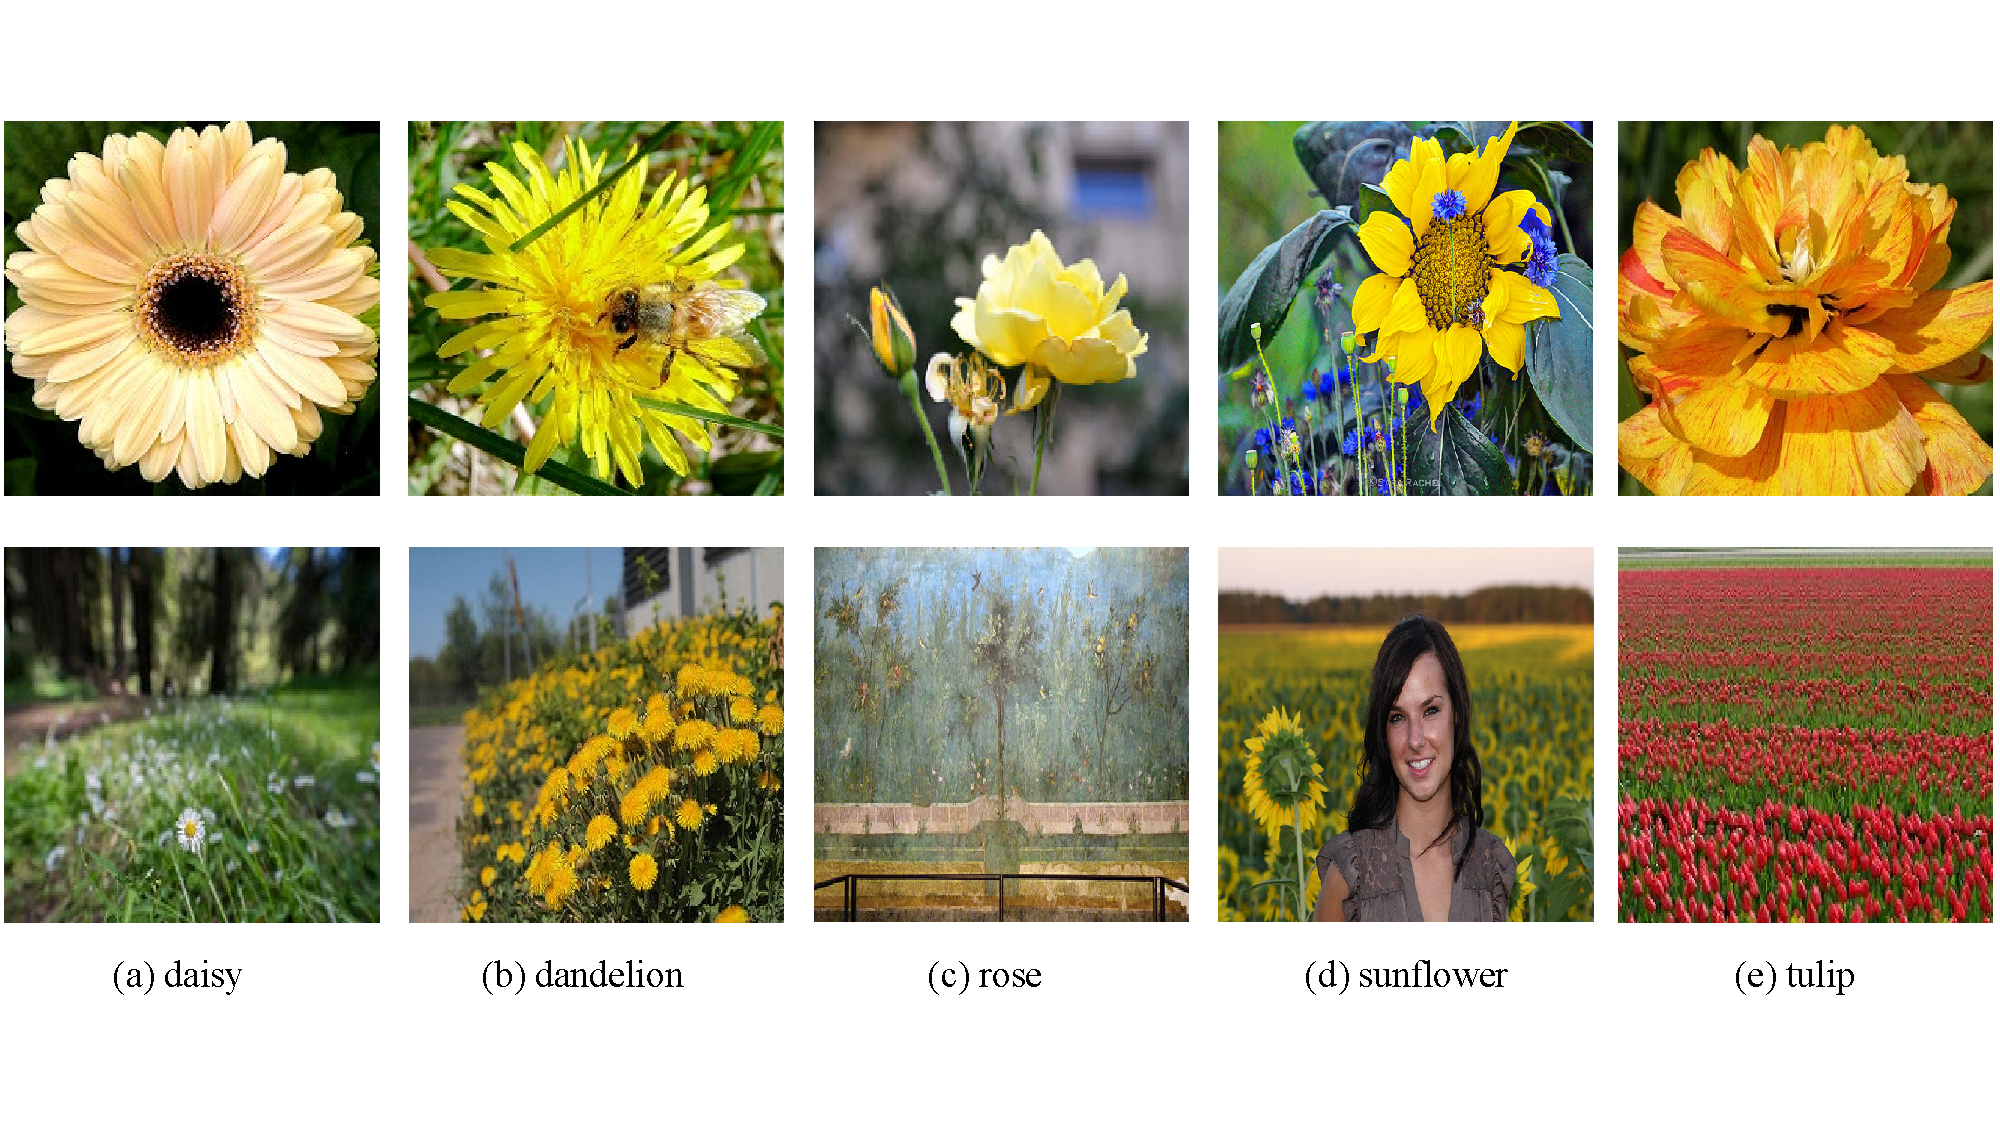
\includegraphics[width=1.0\linewidth]{/Users/malujie/Desktop/latex 2/1.pdf}

   \caption{Original images}
\end{figure}


%------------------------------------------------------------------------
\subsection{Introduction about baseline model}

This baseline uses two convolutional layers to extract features and four fully-connected layers to classify the extracted features.
The problem is that the number of convolutional layers is too small, which leads to inadequate extraction of features, and the number of fully-connected layers is too large, which leads to overfitting of the whole network.

%------------------------------------------------------------------------
\section{Apply Tricking}

Because of many factors in the given dataset will influence the accuracy, so the baseline model do not works good.
For this reason, how to make the neural network learn features without overfitting has become the most important goal of this competition.
Four tricks were adopted to complete this competition as shown:

\textbf{(1)} The network structure of resnet18 is adopted and the redundant fully connected layers in the baseline are discarded in order to learn more discriminative features. ~\cite{https://doi.org/10.48550/arxiv.1512.03385}

\textbf{(2)} The pre-training method is adopted to prevent the resnet18 network from falling into overfitting, and the parameter weights trained on the imagenet dataset can better optimize the entire network parameters.~\cite{https://doi.org/10.48550/arxiv.1905.00546}

\textbf{(3)} Most of the time Adam gets the optimal solution is Sharp Minimum, and SGD gets Flat Minimum, which is why we set optimizer to SGD.~\cite{https://doi.org/10.48550/arxiv.2002.07839}

\textbf{(4)} The imagenet dataset is very large, so the provided flower dataset and the flower samples in the imagenet dataset have high similarity, and the number of samples in the provided dataset is also relatively large, so different learning rates are adopted in different Network layers.~\cite{10.5555/1756006.1756025}


%------------------------------------------------------------------------
\section{Experiment analysis}

Four tricks were adopted in this competition, so ablation experiments have been done to verify the effectiveness of each trick. 
The effectiveness of various tricks obtained through ablation experiments are shown in Table 1. 
Trick1 adopts the network structure of resnet18, trick2 adopts the pre-training model, trick3 adopts the SGD optimizer, and trick4 adopts different learning rates for different network layers. 
As can be seen from Table 1, the four adopted tricks have achieved good results, and the entire model has learned more discriminative features.

\begin{table}[htb]
	\begin{center}
		\caption{Accuracy -- Tricks}
		\label{table:1}
		\begin{tabular}{|c|c|c|c|c|}
			\hline   \textbf{Trick1} & \textbf{Trick2} & \textbf{Trick3} &  \textbf{Trick4} & \textbf{Accuracy}\\
			\hline   N & N & N & N & 71.3\%  \\
			\hline   Y & N & N & N & 75.6\% \\
			\hline   Y & Y & N & N & 86.1\% \\
			\hline   Y & Y & Y & N & 88.7\% \\
			\hline   Y & Y & Y & Y & 92.6\% \\
			\hline
		\end{tabular}
	\end{center}
\end{table}

More intuitive observations can be made in Figure 2 and Figure 3. 
Figure 2 represents the accuracy curve and the Figure 3 represents the loss curve after applying the different tricks respectively.

%---- figure part -------
\begin{figure}[htp]
  \centering
  %\fbox{\rule{0pt}{2in} \rule{0.9\linewidth}{0pt}}
   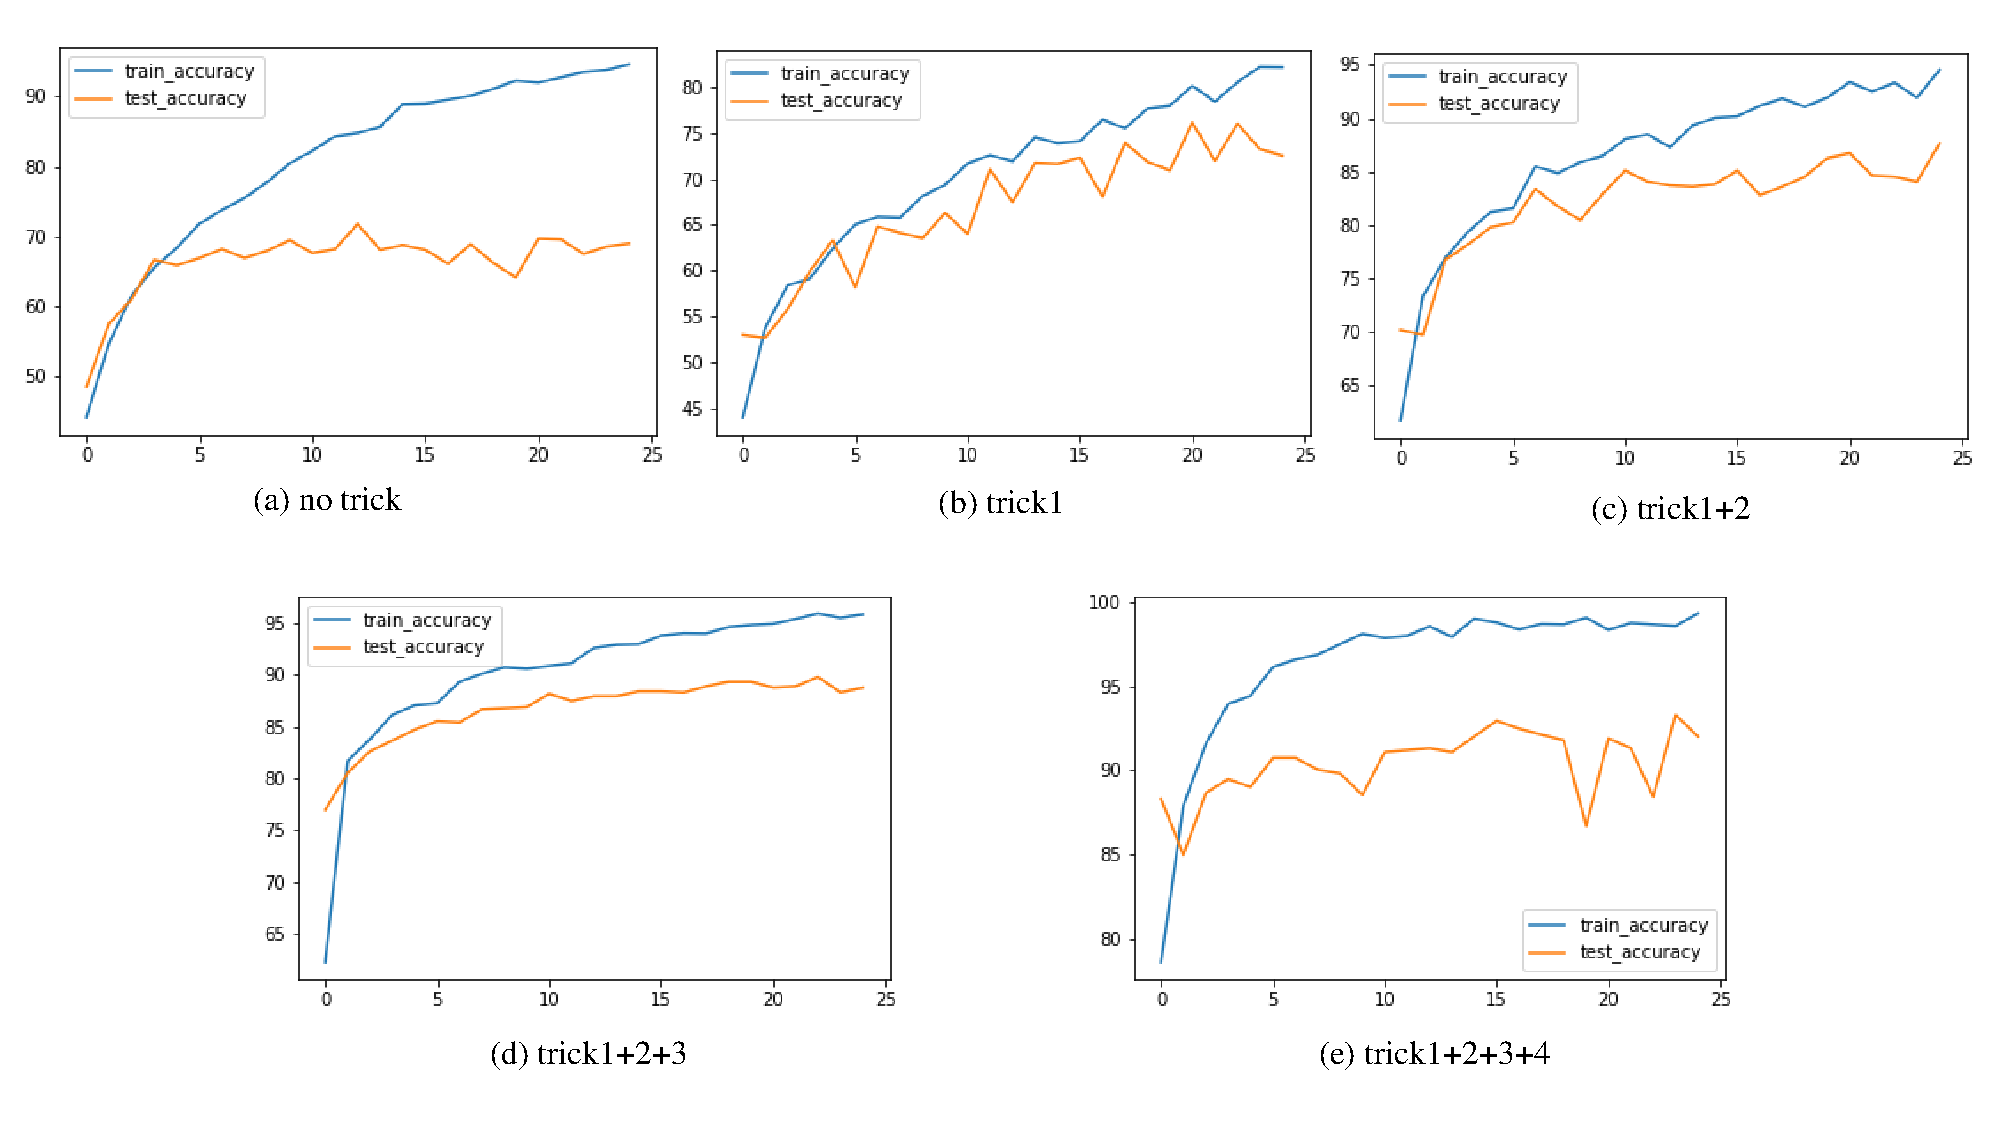
\includegraphics[width=0.9\linewidth]{/Users/malujie/Desktop/latex 2/2.pdf}

   \caption{Accuracy under different tricks adopted}
\end{figure}


%---- figure part -------
\begin{figure}[htp]
  \centering
  %\fbox{\rule{0pt}{2in} \rule{0.9\linewidth}{0pt}}
   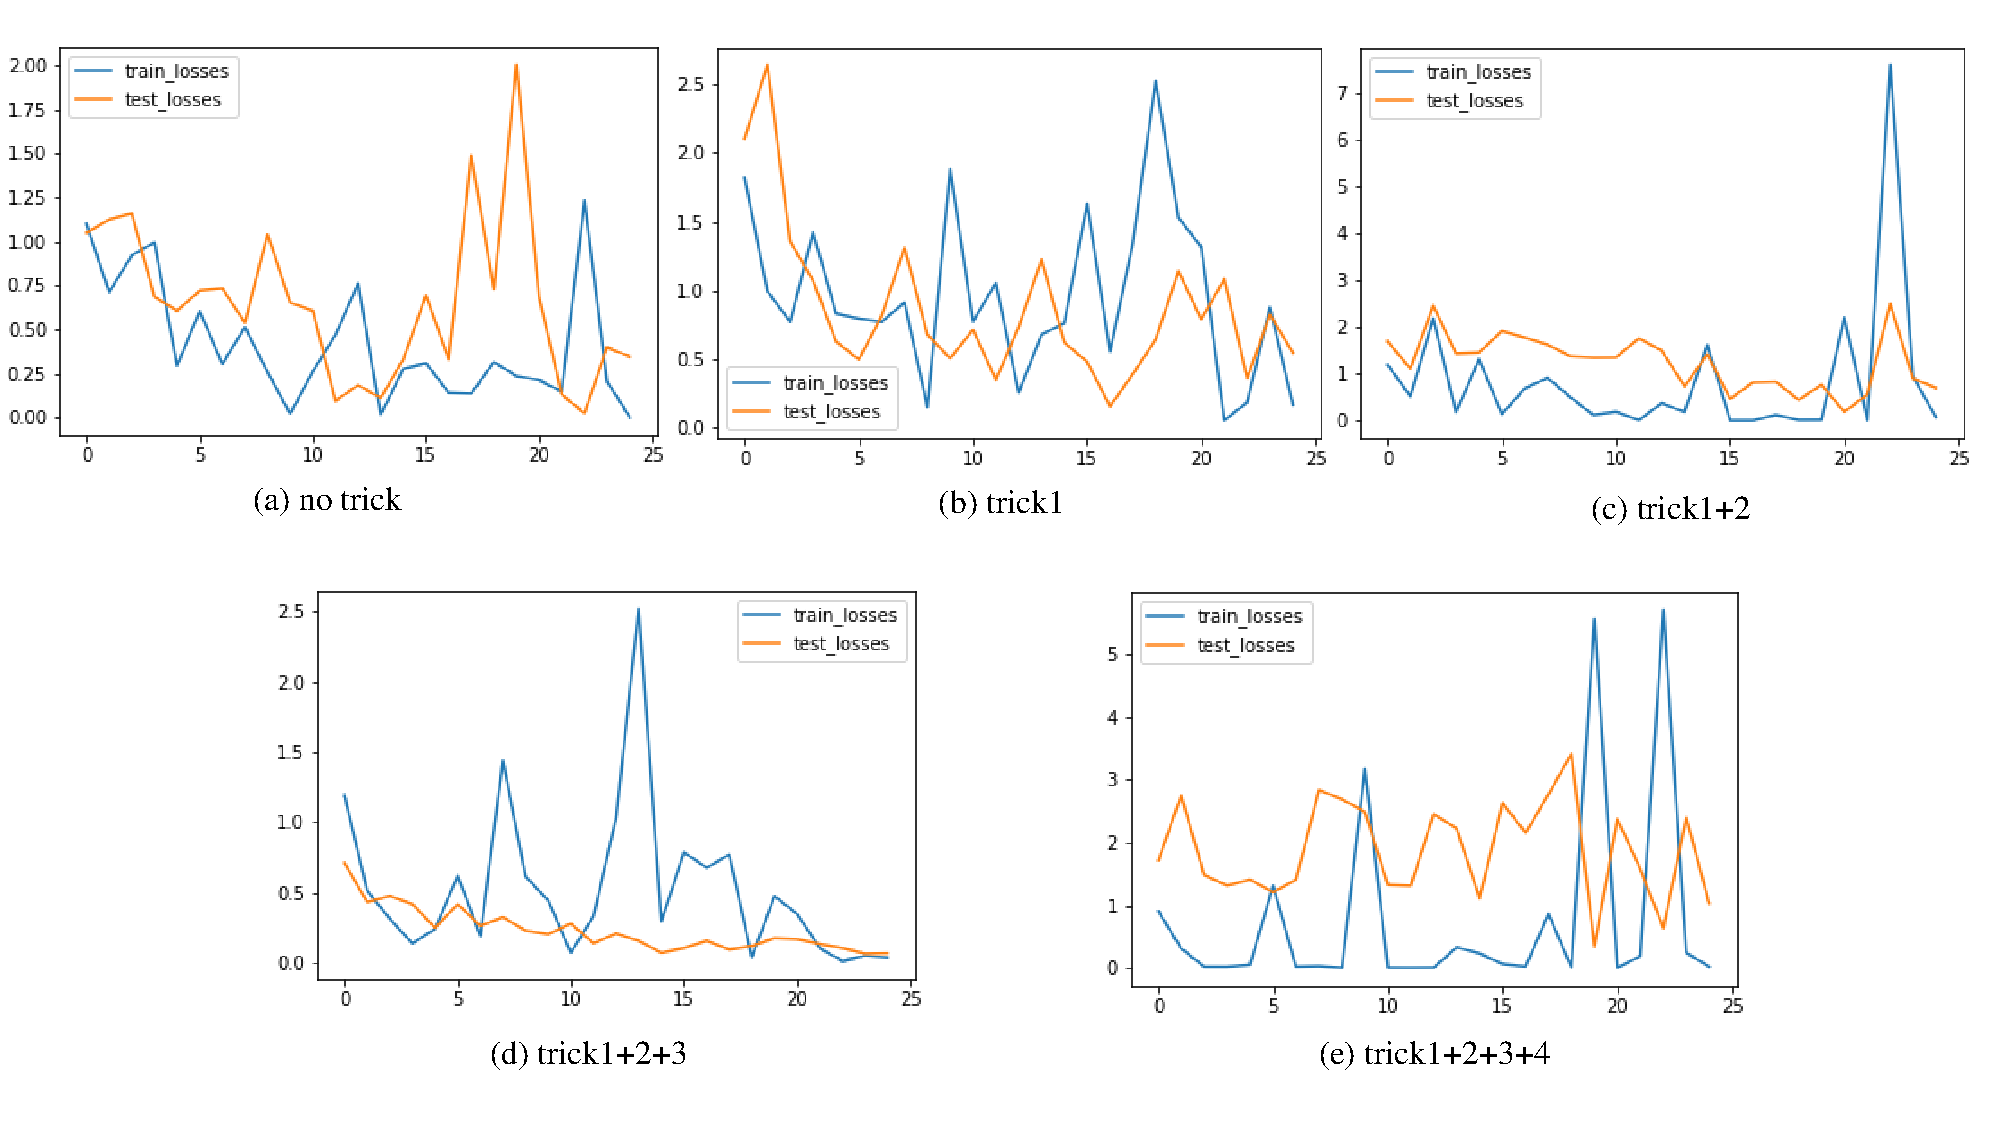
\includegraphics[width=0.9\linewidth]{/Users/malujie/Desktop/latex 2/3.pdf}

   \caption{Losses under different tricks adopted}
\end{figure}

%------------------------------------------------------------------------
\section{Observation}
As shown in Figure 2, the training accuracy of the baseline is rising, while the test accuracy is falling, and the difference between the accuracy is getting higher and higher. This shows that the baseline easily falls into overfitting, and the entire network does not learn good features. As can be seen from Figure 3, the test loss in the baseline fluctuates greatly in the later stage, indicating that the generalization of the baseline is poor. The adopted series of methods can solve the above problems well, the network has learned more discriminative features, and the generalization of the network has also been improved.

%------------------------------------------------------------------------
\section{Conclusion}
Flower classification is a task of fine-grained image classification. Fine-grained images have large intra-class differences and small inter-class differences. How to learn more discriminative features is the core of this task. For this reason, the deeper network resnet18 was adopted, and the pre-training method with different learning rates on different layers and SGD optimizer were adopted to improve the efficiency of the entire network. The final classification accuracy reached 92.6\%, and the flops was 3.59G.

%------------------------------------------------------------------------
\section{Final}
You can check our code in our Github  respositories:
\url{https://github.com/XiaoLinZzz/CV-project}.


%%%%%%%%% REFERENCES
{\small
\bibliographystyle{ieee_fullname}
\bibliography{sample}
}

\end{document}
